\begin{savequote}[75mm]
Does this shit even work?
\qauthor{A Tired Grad Student}
\end{savequote}

\chapter{High-throughput behavior in rats}

\newthought{The laboratory rat \textit{Rattus norvegicus}} was the first mammalian species domesticated for scientific research\cite{Jacob199}, and has since been the most widely studied specie in biomedical research. In the lab, rats can be trained to perform cognitively demanding tasks. They have a long history as laboratory models for the behavioral study of cognitive capacities, including decision-making\cite{Brunton2013, REFREF}, working memory\cite{REFREF}, memory consolidation\cite{REF}, and spatial navigation\cite{REFREF}. 

One of the most widely used tools for studying animal behavior in the lab is the operant conditioning chamber\cite{REFREF}. With the conditioning chamber, the experimenter gradually shapes the animal's behavior until the desired task is learned. Like most rodent behavior experiments, tests of visual object recognition rely on operant conditioning. In 1930, Karl Lashley\cite{Lashley1930} described a wide range of visual behaviors in rats using what is now a classic two-choice paradigm\ref{fig:FIG?}. In his version of the rig, Lashley tested rats' visual shape recognition capacities by training them to select a particular gate or door depending on what stimulus it showed in order to access a hidden food reward. 

Fast-forward ~80 years, experiments have relied on similar training rigs to test rats on visual object recognition tasks\cite{Zoccolan2009, ETC}. 

Technological developments over the past ten years have enabled experiments to use these traditional conditioning boxes in computer-controlled systems that allow for automated and high-throughput training. 

Automated training methods are more efficient because they require little to no hands-on involvement from the experimenter. Animals can be placed into chambers by staff who are unbiased about the particular study's goals or they can simply live in the boxes with automatically or remotely controlled training regimes\cite{MouseAcademy, Raj, Brody}. Thus, high-throughput systems not only allow for more systematic and less biased experiments, but importantly, they also allow many animals to be trained and studied in parallel. Higher-throughput studies provide statistical power difficult to achieve with small-scale animal cohorts and importantly, have the potential to provide a readily available source of animals for physiological access or perturbation studies.

The advantages of automated, high-throughput systems become particularly important for behavioral tasks that are complex and require long training schedules.  

% This is a math equation that can go here for now.
% $$\zeta = \frac{1039}{\pi}$$

% %%%%%%%%%%%%%%%%%%%%%%%%%%%%%%%%%%%%%%%%%%%%%%%%%%%%%%%%%
% OpenRatBox
% %%%%%%%%%%%%%%%%%%%%%%%%%%%%%%%%%%%%%%%%%%%%%%%%%%%%%%%%%
\section{OpenRatBox: An open-source platform for high-throughput behavior}
One major advantage of rodents over primates is that their smaller size allows many more animals to be studied at once. While most studies using monkeys rely on about 2-3 animals (though see \cite{REFREF} developmental stuff), standard rat studies use ~4-6 animals per experiment\cite{REFREF}, while mouse studies use ~10-20 animals\cite{REFREF}. 

These sample counts have exploded with the development of computer-controlled, automated training systems described above. Inspired by the work of Brody, Scott, Olveczky, and colleagues, we developed a high-throughput behavioral apparatus for visual behavior tasks in rats. We sought to make a system that was reproducible, low-cost, and modular. 

It was critical to design training boxes that would be straightforward to reproduce, not only to maintain constancy from one box to the next, but also to facilitate widespread use both within the lab and across labs. Systematization across research groups can be immensely powerful, especially for studying highly complex, multi-modal processes like decision-making, as exemplified by the International Brain Laboratory\cite{IBL} and the Allen Brain Institute\cite{REFREF}.

In order to build behavior boxes at a larger scale, we relied on low-cost, readily accessible components and open-source software for experimental control. While it is possible to build a highly sophisticated and customized apparatus that meets the particular demands of a given experiment, it can be extremely costly and hard to adapt for other experiments or impossible to use by other labs. In contrast, designing a low-cost system that relies on open-source technology allows it to be more accessible as a tool that can benefit others, while also allowing for continued improvements and new adaptations. 

Modularity is important because a given behavior can be tested under different regimes. For example, two commonly used behavior choice paradigms are Go/No-Go (GNG) and two-alternative forced choice (2AFC) tasks. These paradigms offer different advantages and disadvantages (see X), and also have different hardware requirements. GNG just requires one choice manipulandum, while 2AFC requires at least two.

% FIGURE 1.1 OpenRatBox Schematic
\begin{figure}[t!]
    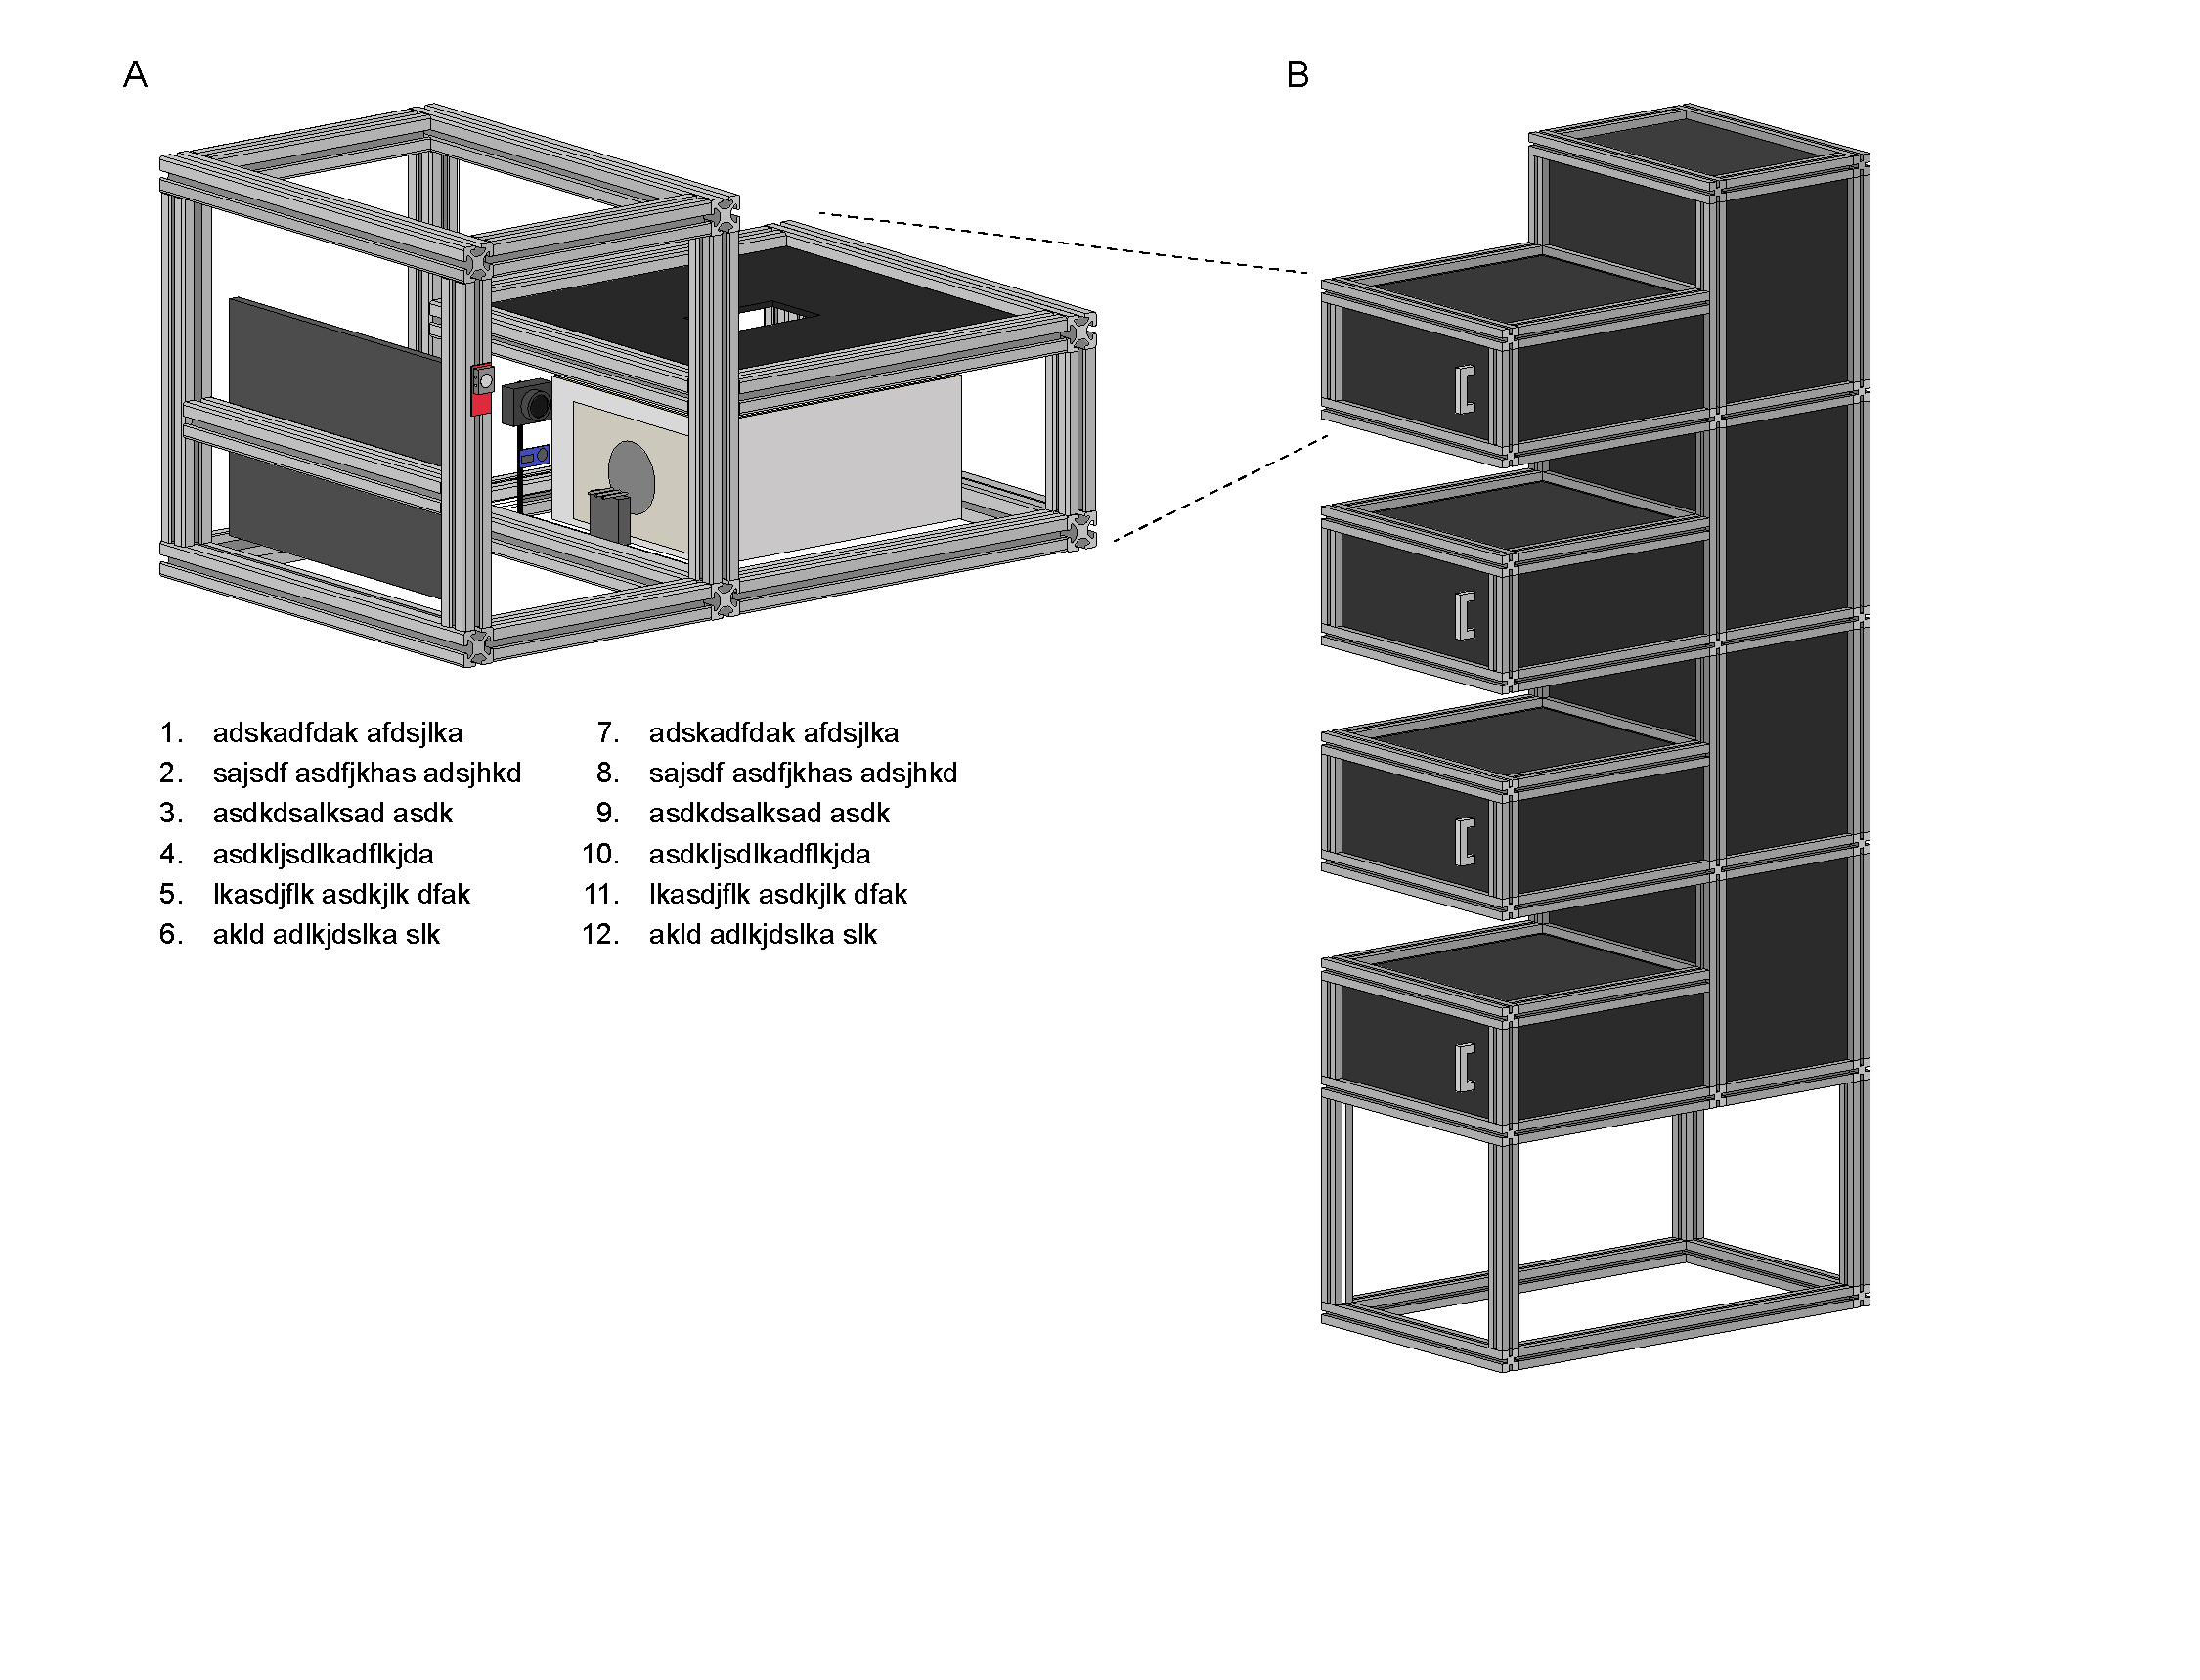
\includegraphics[width=\textwidth]{figures/chapter_1/fig_1-1_openratbox/openratbox.pdf}
    \vspace{.1in}
    \caption[OpenRatBox]{OpenRatBox: Open-source, automated, high-throughput training. \textbf{A.} One training box. Parts: 1. Home cage, 2. Sensors and reward ports, 3. USB camera and IR detector, 4. Monitor, 5. Solenoid valves, 6. Tubing and wiring leads out of the vestibule, etc. \textbf{B.} A full tower assembly of four identical training boxes. 
    \label{fig:openratbox}}
\end{figure}

The overall design of each box is identical, and experiment-specific adjustments are made with modular components. The main vestibule of each unit houses the animal's cage and all hardware needed to collect the animal's response and monitor its behaviors (Figure\ref{fig:openratbox}\textbf{A}). Each unit is equipped with a small computer that allows as many experiments to be run independently and in parallel as there are boxes. 

The external frame is composed of aluminum extrusion bars and custom-cut acrylic paneling that fits into the railing slots of the bars, such that an arbitrary number of boxes can be built on top of the next, limited by the available vertical space (Figure\ref{fig:openratbox}\textbf{B}). All the training boxes are controlled and monitored by a control computer that runs a client (MWorks) that interfaces with the servers running in each behavior box. 

Within a given unit, there are two partitions. The monitor is mounted on a partition separate from the main vestibule in order to keep it clean and protected (for example, from chewing, or stray water droplets and bedding). The animal has visual access to the monitor through a window separating the monitor from the main vestibule that holds the cage. 

The cage itself is held in place with two spring-loaded latches that allow the cage to be loaded into the same relative position, if necessary. The cage locking mechanism was adapted from a commercially available, self-standing animal cage rack, in which each cage is locked into the air circulation and filtration system. The box is thus designed to support fully live-in animal behavior training. 

Mini extrusion bars (REFREF) are screwed directly into strategic positions on the acrylic floor of the main vestibule. This effectively creates a mountable rail system for attaching experiment-specific components, such as reward ports, USB cameras, and IR detectors (see Figure\ref{fig:box_components} REFREF). As such, any modifications specific to a paradigm (\textit{e.g.}, one reward port or three reward ports) could be easily attached or removed from one box to the next. All wiring feeds through small access holes cut into the acrylic pieces embedded into the extrusion bars, as does tubing for water delivery of rewards. Attached to each box is a small computer (Mac Mini, though others are possible) that runs the experiment (visual stimulation, I/O control, and so on). 

\section{High-throughput training}
% FIGURE 1.2 Basic 2-choice task, high throughput

% fig:

We tested a Go/No-Go (GNG) paradigm and a two-choice paradigm, as each offers different advantages and disadvantages. In Go/No-Go (GNG) paradigms, the animal responds to a given stimulus (the "Go" condition) by licking a choice port or pressing a lever, and must withhold a response otherwise (the "No-Go" condition). GNG paradigms have fewer moving parts, requiring only one response type, which can make it easier to learn. However, subjects tend to make more Go responses in the GNG task, as the Go response is rewarded while other other behaviors are not\cite{REFREF}. 

For physiology experiments, GNG paradigms are more amenable to head-restrained animals, since the animal only needs to make one type of response. On the other hand, since reward strongly modulates neural activity, and GNG paradigms can be challenging as the stimulus, response, and reward are tightly linked\cite{REFREF}. Multi-port tasks, like two-choice paradigms, overcome many of these drawbacks, as the animal is trained to respond in one way to condition A and some other way to condition B. In this way, the stimulus, response, and reward can be disentangled, but at the cost of a more complicated task structure that can make interpretations difficult in still other ways. However, they can be more difficult to adapt for head-restrained conditions. Animals normally use head movements or their whole body to reach one reward port or the other\cite{REFREF}, which is not possible in physiology experiments that require the animal's head to be fixed in place in the recording apparatus. 



We trained rats to perform a simple two-category object discrimination task. Animals had to lick one response port for object ``A'', and another response port for object ``B''.  Animals could be trained to perform basic shape discriminations for reasonably dissimilar objects (\textit{e.g.} the objects in FIGUREXREFREF) in one month or less, and animals readily performed several hundred trials per day in the automated training rig. 

\section{Generating complex visual object stimuli}
Morph stimuli and stuff

% FIGURE 1.3 Stimulus generation

\section{Tests of visual object discrimination and recognition}
% FIGURE 1.3 INVARIANCE TEST

After learning the ``base'' object A/B task, animals were presented with two types of generalization tests. In the first, INVARIANT OBJE RECT.

% FIGURE 1.4 MORPHS
In the second test, samples from a morph line between the previously trained ``poles'' of the stimulus continuum. REFREF shows two-dimensional stimuli generated using closed non-uniform rational B-spline curves interpolating smoothly in the space of their control vertices. 

During the ``probe'' phase of the task, morphed samples were randomly interleaved roughly 10\% of the time, without feedback, during the ordinary discrimination task. These probe trials were then used to build up a psychophysical curve to determine the animals' naive behavior in classifying the objects as ``A'' or ``B''. 

These curves characterize the category boundary along the morph axis 


\begin{figure}
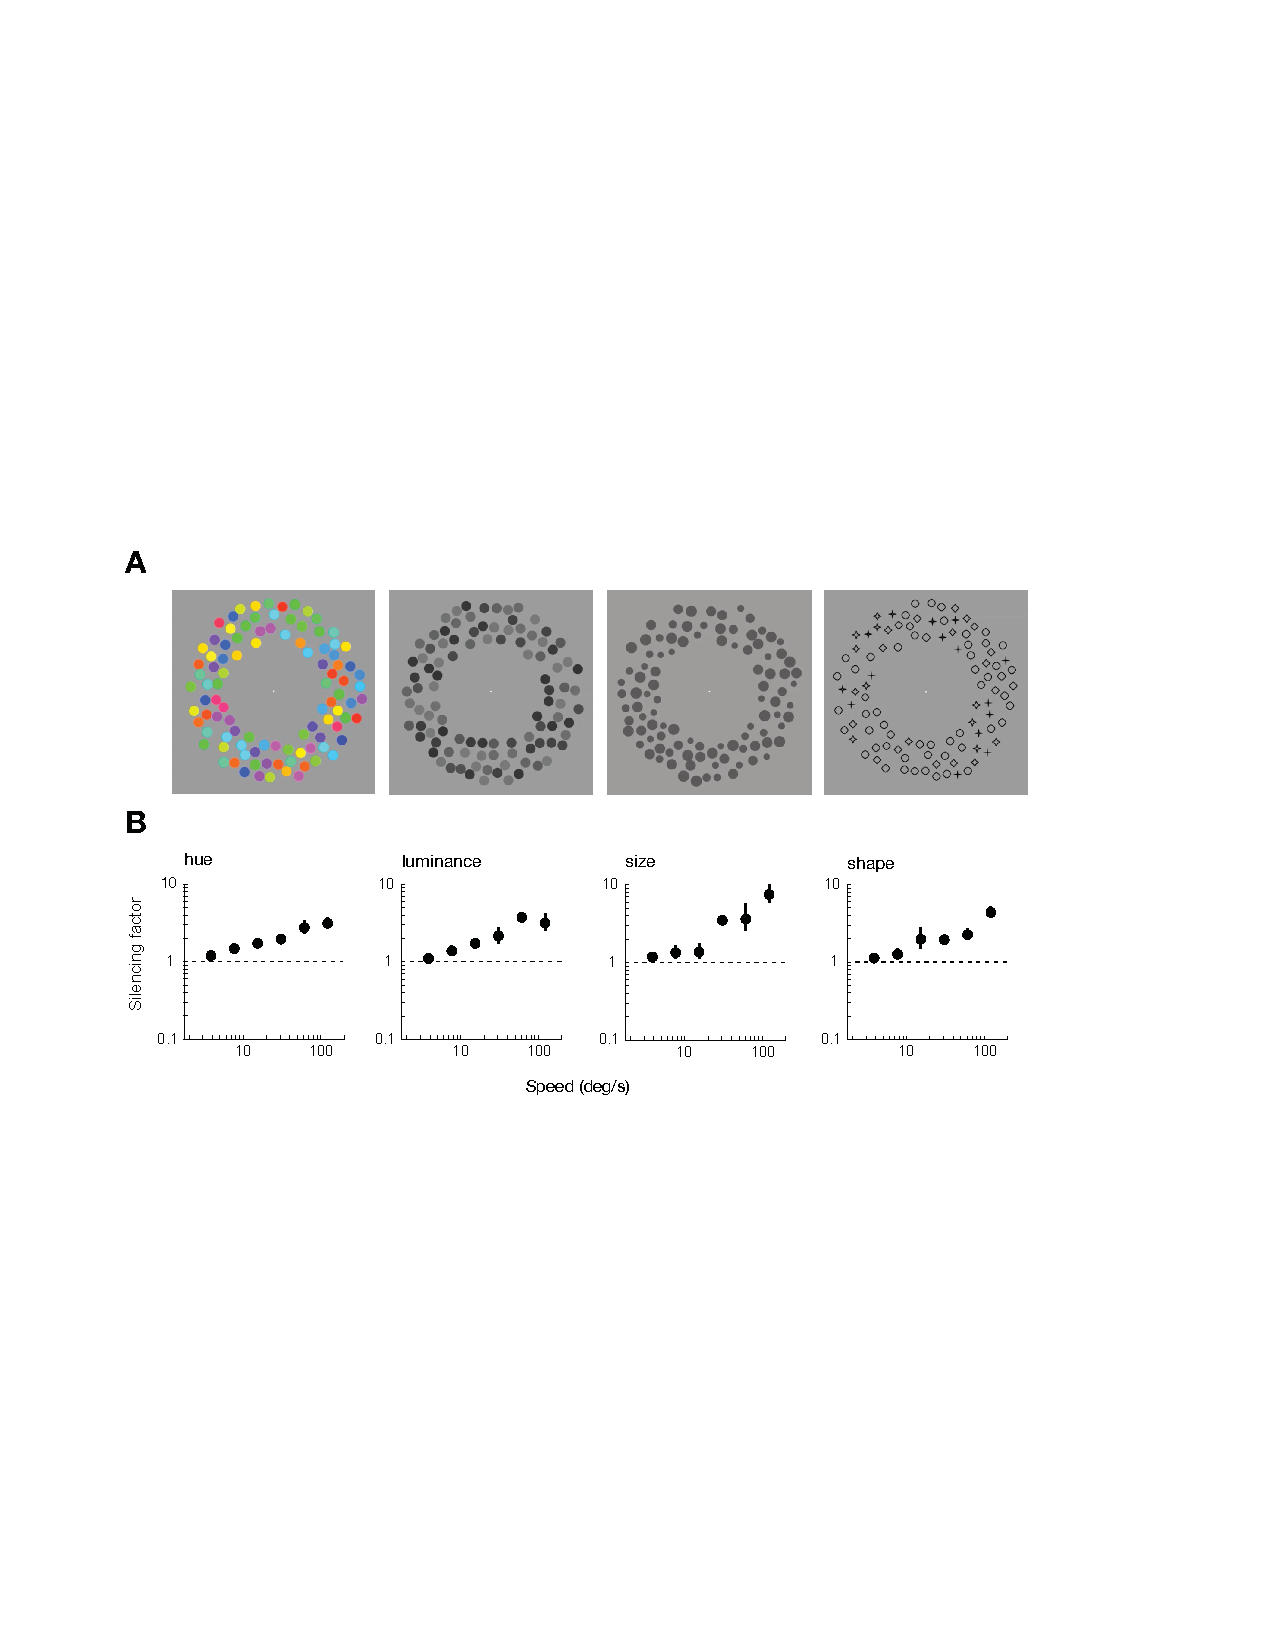
\includegraphics[width=\textwidth]{figures/fig1}
\caption[Short figure name.]{This is a figure that floats inline and here is its caption.
\label{fig:myInlineFigure}}
\end{figure}

Stuff can be written here



% \texttt{This is a line of code.}


% For an example of a full page figure, see Fig.~\ref{fig:myFullPageFigure}.

% % EXAMPLE FIGURE 
% \begin{figure}[t!]
%     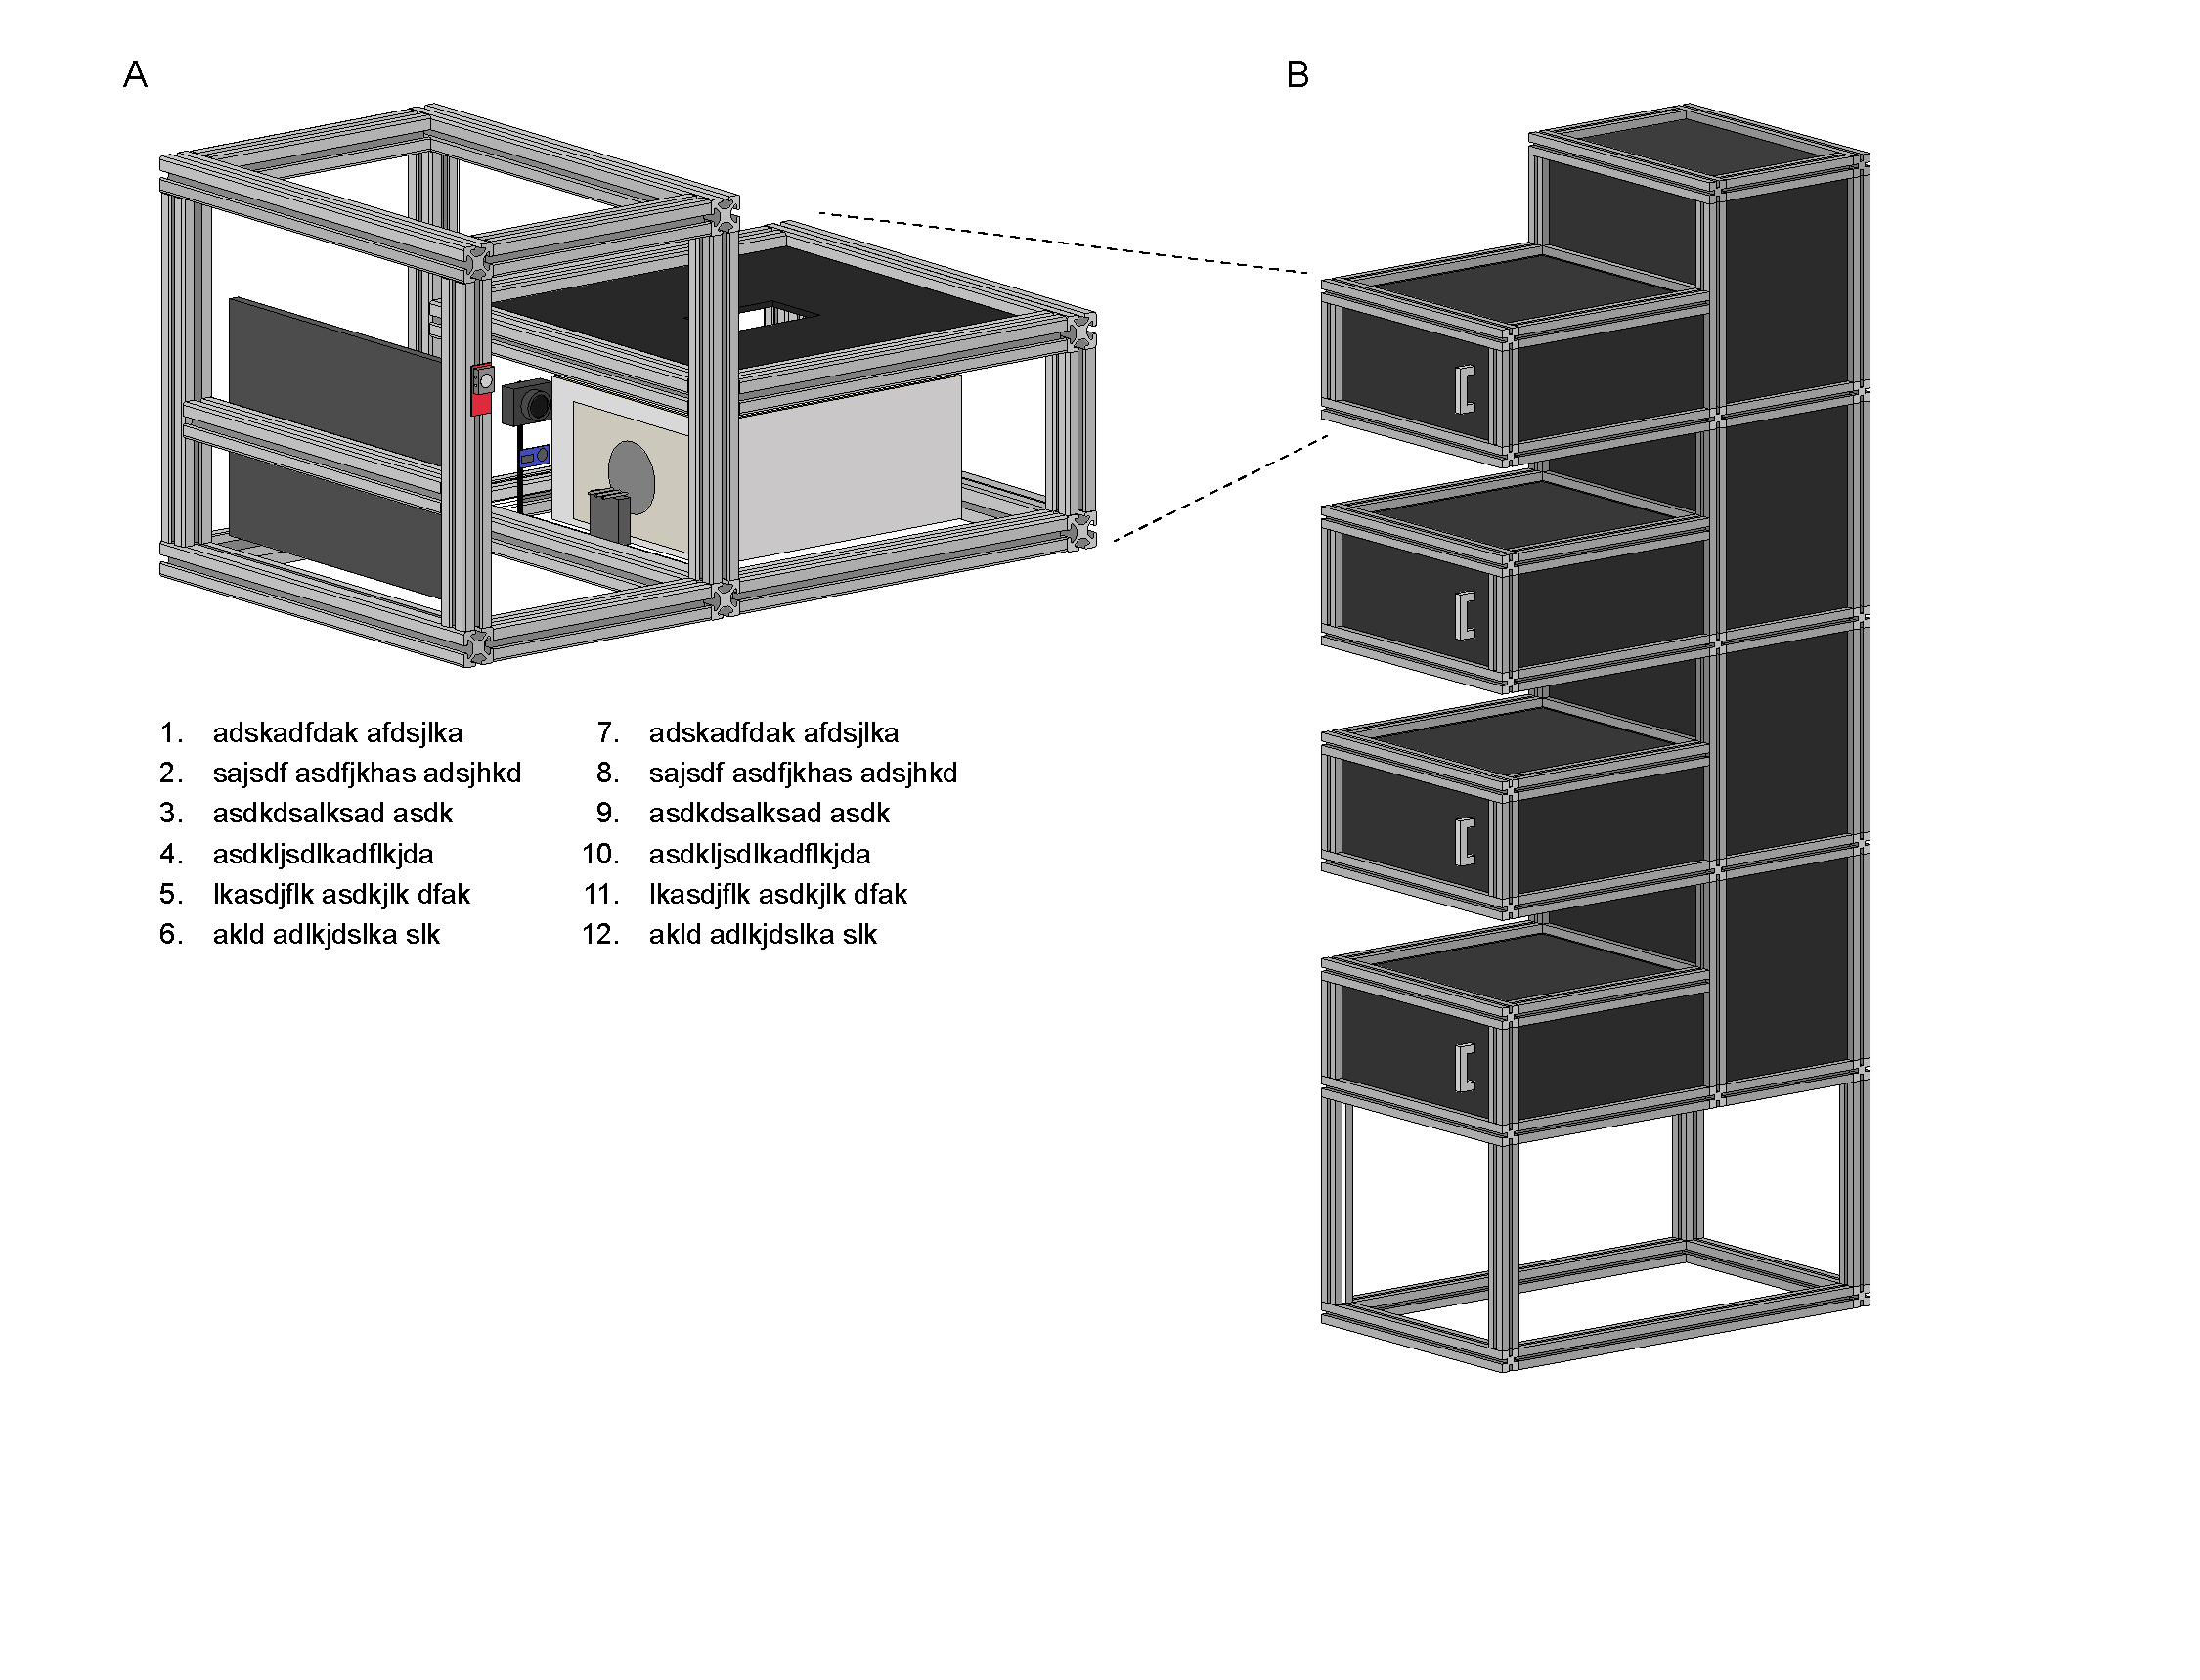
\includegraphics[width=\textwidth]{figures/chapter_1/ratbox_schematic.pdf}
%     \vspace{.1in}
%     \caption*{\textbf{Figure 2.1} Example figure and tips -- A) Your figure numbers should follow the format of Figure chapter#.figure#. B) Set width equal to textwidth. C) Specify position as [t!] to insert at page top.}
% \end{figure}

%% Requires fltpage2 package
%%
% \begin{FPfigure}
% 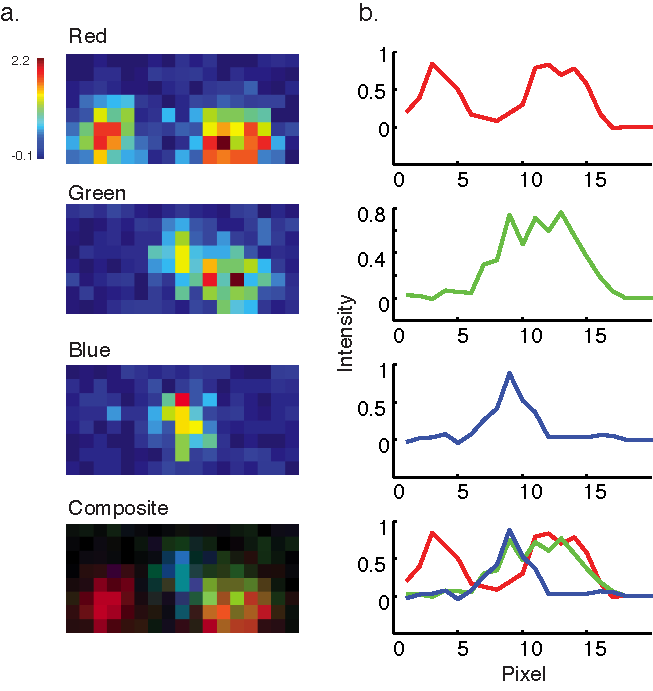
\includegraphics[width=\textwidth]{figures/fullpage}
% \caption[Short figure name.]{This is a full page figure using the FPfigure command. It takes up the whole page and the caption appears on the preceding page. Its useful for large figures. Harvard's rules about full page figures are tricky, but you don't have to worry about it because we took care of it for you. For example, the full figure is supposed to have a title in the same style as the caption but without the actual caption. The caption is supposed to appear alone on the preceding page with no other text. You do't have to worry about any of that. We have modified the fltpage package to make it work. This is a lengthy caption and it clearly would not fit on the same page as the figure. Note that you should only use the FPfigure command in instances where the figure really is too large. If the figure is small enough to fit by the caption than it does not produce the desired effect. Good luck with your thesis. I have to keep writing this to make the caption really long. LaTex is a lot of fun. You will enjoy working with it. Good luck on your post doctoral life! I am looking forward to mine. \label{fig:myFullPageFigure}}
% \end{FPfigure}
% \afterpage{\clearpage}

